\documentclass[titlepage]{article}
\usepackage[left=2.54cm,top=2.54cm,right=2.54cm,nohead]{geometry}
\usepackage{graphicx}
\title{ECE354 System Design Document}
\author{
Group Number: 01\\\\
Group Members:\\
\begin{tabular}{|l|c|c|}
\hline
Name & UWID & Student ID\\
\hline
Kim, Yubin & y12kim &20239608\\
Burstyn, Daniel & dmbursty &20206120\\
Collins, Joseph & j4collin &20222997\\
Flath, Nathaniel & nflath &20252804\\
\hline
\end{tabular}
}
\begin{document}
\maketitle
\newpage
\tableofcontents
\newpage

\section{Introduction}

This document describes the basic functionality of the Real-Time Operating
System to be implemented by this group.  Included in this document are a list of
public and private primitives and pseudocode for these methods, kernel-level
variables, and default processes.  Also included in this doument are plans to
set up and handle hardware and software interrupts, as well as our
implementation and testing strategies.\\
\\
This operating system will have 8 public primitives, all of which will be
represented by user-level function and a corresponding kernel-level function.
When a process calls the user-level function, the function will `trap' into the
kernel-level function---that is, it will cause a software interrupt. The
handler for the software interrupt will call \verb!bridge!,
which is the connection between user-level and the kernel-level.  The following
describes the relationship between the various kernel-level functionalities.

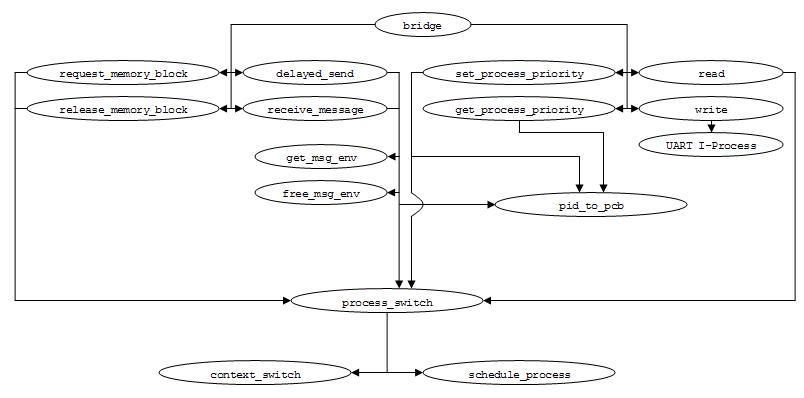
\includegraphics[width=15cm]{dependency.jpg}

The operating system will also use its 1 MB of memory, organized roughly in the following manner:

\begin{center}
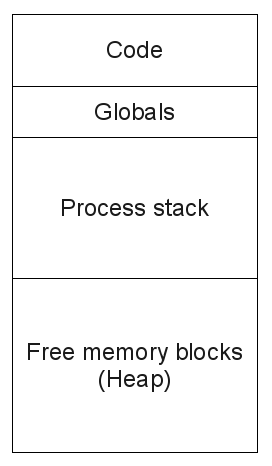
\includegraphics[height=7.1cm]{memorymap.png}
\end{center}

Note that the sizes of the blocks of memory are not to scale. Exact numbers for
the blocks of memory will be determined when the RTX is initialized.

\section{Global Information}

\subsection{Variables}

\subsubsection{UART Buffers}
\begin{tabular}{ll}
\verb!char[128] uart_read_buffer!     & A circular buffer containing the characters ready to be read from the UART.\\
\verb!short[2] uart_read_buffer_loc!  & The locations of the first valid character in the buffer and one past the last\\
                                      & valid character.\\
\verb!char[128] uart_write_buffer!    & A circular buffer of characters to write to the console.\\
\verb!short[2] uart_write_buffer_loc! & Locations of the first valid character, and one past the last valid character\\
                                      & in the buffer.
\end{tabular}

\subsubsection{Process Queues}
Where an array of PCB lists are given, they represent one index per priority
level.\\\\
\begin{tabular}{ll}
\verb!PCB_list*[5] malloc_blocked_processes! & List of processes waiting for memory.            \\
                                             & Each array location stores a different priority. \\
\verb!PCB_list* uart_blocked_processes!      & List of processes waiting for UART input.       \\
\verb!PCB_list* message_blocked_processes!   & List of processes waiting for messages. \\
\verb!PCB_list*[5] ready_processes!          & List of processes ready for execution.
\end{tabular}

\subsubsection{Other Variables}
\begin{tabular}{ll}
\verb!unsigned int current_time! & The number of milliseconds the OS has been running.\\
\verb!PCB[] pcb_map! & Map of all processes to their process IDs.\\
\verb!int num_processes! & Number of processes.\\
\end{tabular}

\subsection{Constants}

\subsubsection{Process IDs}
\begin{tabular}{ll}
\verb!KCI_PID! & Process id for the KCI \\
\verb!KCD_PID! & Process id for the KCD \\
\verb!NULL_PID! & Process id of the null process \\
\verb!UART_IPROCESS_PID! & PID of the UART I-Process \\
\verb!TIMER_IPROCESS_PID! & PID of the Timer I-Process \\
\verb!DUMMY_PID! & An invalid dummy process id \\
\end{tabular}
\subsubsection{Process Statuses}
\begin{tabular}{ll}
\verb!ST_EXECUTING! & Currently executing \\
\verb!ST_READY! & Ready to execute \\
\verb!ST_BLOCKED_ON_UART! & Blocked on read from UART \\
\verb!ST_BLOCKED_ON_MESSAGE! & Blocked on recieve message \\
\verb!ST_BLOCKED_ON_MEMORY! & Blocked on get memory block \\
\verb!ST_ZOMBIE! & Finished execution or encountered exception\\
\end{tabular}
\subsubsection{Message Types}
\begin{tabular}{ll}
\verb!KC_MSG_TYPE! & Keyboard command from KCI to KCD \\
\verb!COMMAND_MSG_TYPE! & Command to be sent to registered process \\
\verb!PRINT_MSG_TYPE! & Print message for CRT display process \\
\verb!TIMER_MSG_TYPE! & Timer update message \\
\end{tabular}
\subsubsection{Return Types}
\begin{tabular}{ll}
\verb!RTX_SUCCESS! & Successful execution \\
\verb!RTX_ERROR! & An error occured \\
\end{tabular}
\subsubsection{Miscellaneous}
\begin{tabular}{ll}
\verb!TIMER_DEV_ID! & Device id of the timer \\
\verb!UART_DEV_ID! & Device id of the UART \\
\verb!TRUE! & 1, for convenience \\
\verb!FALSE! & 0, for convenience \\
\verb!void* NULL = 0! & The null pointer \\
\end{tabular}

\subsection{Data Structures}
\subsubsection{List}
A list is a linked list containing values of a specified type.  The list
structure will be as follows:\\
\begin{verbatim}
struct list
{
    object object; //Object represents the type of object represented by this list
    list* next;
};
\end{verbatim}

The following functions will be implemented for list types:\\\\
\verb!void list_add_at_end(list*, object)! - This function adds the given object to
the end of the list.\\
\verb!void* list_get(list*, int n)! - This function returns the $n^{th}$ object in the
list.  If list has fewer than n objects, it returns a sentinel.

\subsubsection{PCB}
The Process Control Block (PCB) will contain data pertaining to a given process.
\begin{verbatim}
struct PCB
{
    int pid;
    int priority;
    int state;
    int is_i_process;
    msg_envelope_list* msg_queue;
    int data_reg[8];
    int add_reg[8];
    int pc; //program counter
    int sp; //stack pointer
    int[2] stack_space; //0 = start, 1 = end
};
\end{verbatim}

\subsubsection{Message Envelope}
Message envelopes will contain data pertaining to the sending of messages between processes.

\begin{verbatim}
struct msg_envelope
{
    int sender_id;
    int dest_id;
    int msg_type;
    void* message;
    int send_time;
};
\end{verbatim}

\section{Primitives}
All of these primitives are run in kernel level and are accessible to user-level
processes via a user-level API.

\subsection{request\_memory\_block}
This primitive returns a free memory block to the calling process.  If there are
no free memory blocks, then the calling process is blocked until one becomes
available.  This function relies upon the \verb!malloc_blocked_process! global
variable and the \verb!process_switch! kernel function.

\begin{verbatim}
void* request_memory_block(void):
begin:
    atomic(on)
    j = -1
    for i from 1 to free-memory[0] while j == -1:
        if memory[i] == 1:
            j = i
        end if
    end for
    if j == -1:
        current_process->state = ST_BLOCKED_ON_MEMORY
        list_add_at_end( malloc_blocked_process[current_process->priority], current_process )
        process_switch()
        goto begin
    end if
    memory[j] = 0
    atomic(off)
    return convert_index_to_pointer(j)

void* convert_index_to_pointer(int j):
    return (void*) (j * size_of_memory_blocks + heapStart)
\end{verbatim}


\subsection{release\_memory\_block}
This primitive frees a memory block, allowing it to be used by another process as needed.  If there are any processes waiting for
memory, it chooses the highest-priority one that has been waiting the longest.
This function relies upon the \verb!malloc_blocked_process! global variable and the
\verb!process_switch! kernel function.

\begin{verbatim}
release_memory_block(void* MemoryBlock)
    atomic(on)
    j = convert_pointer_to_index(MemoryBlock)
    memory[j] = 1
    PCB* blocked_process = 0
    for i from 0 to 5 while blocked_process = 0:
        blocked_process = list_get(malloc_blocked_processes[i], 0)
        malloc_blocked_processes[i] = list_get(malloc_blocked_processes[i], 1)
    end for
    if blocked_process != 0:
        blocked_process->state = ST_READY
        if blocked_process->priority > current_process->priority:
          process_switch()
        end if
    end if
    atomic(off)
    return RTX_SUCESS

int convert_pointer_to_index( void* MemoryBlock ):
    return (int)(MemoryBlock - heapStart) / size_of_memory_blocks
\end{verbatim}

\subsection{delayed\_send}
This primitive will attempt to send a message to another process, returning 0 on
success or non-zero on failure.  This function relies on the \verb!current_time! and
\verb!current_process! variables, as well as the kernel functions
\verb!pid_to_pcb!, \verb!process_switch!, \verb!get_msg_env! and \verb!free_msg_env!.

It should be noted that messages sent to a process will be sorted by delivery
time so as to reduce the burden of the Timer I-Process.

\begin{verbatim}
int delayed_send (int process_id, int msg_type, void* Message, int delay)
    msg_envelope_node* newMsg = get_msg_env ()
    if newMsg == NULL then return RTX_ERROR
    newMsg->sender_id = current_process->pid
    newMsg->dest_id = process_id
    newMsg->msg_type = msg_type
    newMsg->message = Message
    newMsg->send_time = current_time + delay

    PCB* receiver = pid_to_pcb (process_id)
    if receiver == NULL:
        free_msg_env (newMsg)
        return RTX_ERROR
    end if
    msg_envelope_list* head = receiver->msg_queue
    if head == NULL OR newMsg->send_time < head->send_time:
        newMsg->next = receiver->msg_queue
        receiver->msg_queue = newMsg
    else:
        while head->next != NULL AND head->next->send_time < newMsg->send_time
            head = head->next
        end while
        newMsg->next = head->next
        head->next = newMsg
    end if

    if delay == 0 AND receiver->state == ST_BLOCKED_ON_MESSAGE:
        receiver->state = ST_READY
        ready_processes[receiver->priority]->add_at_end (receiver)
        if current_process->priority < receiver->priority then process_switch()
    end if
\end{verbatim}

\subsection{receive\_message}

This primitive will attempt to receive a message from another process, blocking
if no message is available.  The exception to this rule is the case of
I-processes, which will return null if no message is available.  This function
relies on the \verb!current_time! and \verb!current_process! variables, as well
as the kernel functions \verb!process_switch!, \verb!get_msg_env! and
\verb!free_msg_env!.

\begin{verbatim}
void* receive_message (int* sender_ID, int* msg_type)
    msg_envelope_list* env = current_process->msg_queue
    while env == NULL OR env->send_time > current_time:
        if (current_process->is_i_process) then return NULL
        current_process->state = ST_BLOCKED_ON_MESSAGE
        process_switch()
        env = current_process->msg_queue
    end while
    current_process->msg_queue = env->next

    if sender_ID != NULL then *senderID = env->sender_id
    if msg_type != NULL then *msg_type = env->msg_type

    void* msg = env->message
    free_msg_env (env)
    return msg
\end{verbatim}

\subsection{set\_process\_priority}
This sets the given process to the given priority level. It will then invoke the
scheduler to see if a higher level process than the current one is now ready. If
so, it will call \verb!process_switch!. If successful, it returns 0. Invalid
inputs return -1. This relies on global variables \verb!current_process! and
private kernel functions \verb!pid_to_pcb! and \verb!process_switch!.

\begin{verbatim}
int set_process_priority (int process_ID, int priority)
    PCB* pcb
    if process_ID != NULL_PID AND priority == 4:
        return RTX_ERROR
    end if
    if process_ID == NULL_PID AND priority != 4:
        return RTX_ERROR
    end if
    pcb = pid_to_pcb(process_ID)
    if pcb == NULL:
        return RTX_ERROR
    end if
    atomic(on)
    int oldPriority = pcb->priority;
    pcb->priority = priority
    if pcb->state == ST_READY:
        remove pcb from ready_processes[oldPriority]
        list_add_at_end(ready_processes[priority], pcb)
    else if pcb->state == ST_BLOCKED_ON_UART:
        remove pcb from uart_blocked_processes[oldPriority]
        list_add_at_end(uart_blocked_processes[priority], pcb)
    else if pcb->state == ST_BLOCKED_ON_MEMORY:
        remove pcb from memory_processes[oldPriority]
        list_add_at_end(memory_processes[priority], pcb)
    end if

    if higher priority process is ready:
        current_process->status = ST_READY
        place current_process on ready queue
        process_switch()
    end if

    return RTX_SUCCESS
    atomic(off)
\end{verbatim}

\subsection{get\_process\_priority}
This primitive returns the priority for the given process id. If successful, it
returns the priority of the requested process. If the process id is invalid, it
returns \verb!RTX_ERROR!. This relies on the private kernel functions
\verb!pid_to_pcb!.

\begin{verbatim}
int get_process_priority (int process_ID)
    PCB* pcb
    pcb = pid_to_pcb(process_ID)
    if pcb == NULL:
        return RTX_ERROR
    end if
    return pcb->priority
\end{verbatim}

\subsection{read}
This primitive is used to read information from one of the two supported devices
--- the UART, and the timer.  The output is written to the given buffer
depending on which device is specified.  Reading from the timer returns the
number of milliseconds the RTX is alive, and reading from the UART returns a
character from the serial port, or blocks until it gets one.\\
\\
\verb!read! depends on the \verb!process_switch! method, which it will call if
it blocks the calling process.  \verb!read! also depends on the global
\verb!uart_read_buffer!, and the global constants \verb!UART_DEV_ID!,
\verb!TIMER_DEV_ID!.

\begin{verbatim}
int read (int device_ID, void * Buffer)
    atomic(on)
    if device_ID == TIMER_DEV_ID:
        *Buffer = current_time
        return RTX_SUCCESS
    else if device_ID == UART_DEV_ID:
        if uart_read_buffer is empty:
            current_process->state = ST_BLOCKED_ON_UART
            put calling process in blocked_on_uart queue
            process_switch()
        else:
            *Buffer = dequeue from uart_read_buffer
        end if
        return RTX_SUCCESS
    end if
    return RTX_ERROR
    atomic(off)
\end{verbatim}

\subsection{write}
This primitive is used to write a null terminated string from the buffer to the
UART.  Should the timer's device id be specified, the primitive should simply
return an error code.\\
\\
\verb!write! does not depend on any functions, however it uses the global
\verb!uart_write_buffer!, and the constants \verb!UART_DEV_ID! and
\verb!TIMER_DEV_ID!.

\begin{verbatim}
int write (int device_ID, void * Buffer)
    atomic(on)
    if device_ID == TIMER_DEV_ID:
        return RTX_ERROR
    else if device_ID == UART_DEV_ID:
        for each char in *Buffer:
            append char to uart_write_buffer
        end for
        trigger UART I-Process
        return RTX_SUCCESS
    end if
    return RTX_ERROR
    atomic(off)
\end{verbatim}

\section{Private Kernel-level Functions}
These functions are not visible to user-level processes and can only be called
by other kernel-level functions such as primitives and interrupt handlers.

\subsection{process\_switch}
This will call \verb!schedule_process! to determine the next process to run, and
then call \verb!context_switch!. Note that changing the current process state
and placing it on different queues will have to be done by the caller. This
relies on the private kernel functions \verb!schedule_process! and
\verb!context_switch!.

\begin{verbatim}
void process_switch()
    PCB* pcb = schedule_process()
    context_switch(current_process, pcb)
\end{verbatim}

\subsection{context\_switch}
This function will save the context of the current process, and loads the
context of the given process, then executes it. This function needs to be atomic
and relies on the global variable \verb!current_process!.

\begin{verbatim}
void context_switch(PCB* current, PCB* next)
    atomic(on)
    save current context
    next->state = ST_EXECUTING
    current_process = next
    restore next context
    asm(RTE)  // this will cause the next process to start running

              // if next had previously called context_switch
    return    // it would start from here.
    atomic(off)
\end{verbatim}

\subsection{schedule\_process}
The scheduler returns the pointer to the PCB of the highest priority process
that is in the ready state. Priority is determined first by the priority level,
then by how long the process was waiting. It depends on the global
\verb!ready_processes! list.

\begin{verbatim}
PCB* schedule_process()
    for each ready_queue by priority level:
        if ready_queue is not empty:
            return list_get(ready_queue, 0)
        end if
    end for
\end{verbatim}

\subsection{pid\_to\_pcb}
This private function takes a process id number and returns the pointer to the
correct PCB. It relies on the global \verb!pcb_map! and \verb!num_processes!. If
the id is invalid, it returns \verb!NULL!.

\begin{verbatim}
PCB* pid_to_pcb(int pid)
    if (pid < 0 OR pid >= num_processes):
        return NULL
    end if
    return pcb_map[pid]
\end{verbatim}

\subsection{get\_msg\_env}
This primitive will allocate a message envelope to a process, or return
\verb!NULL! if none are available.  It relies on the variable
\verb!msg_envelopes!.

\begin{verbatim}
msg_envelope_node* get_msg_env (void)
    atomic(on)
    if msg_envelopes == NULL:
        atomic(off)
        return NULL
    end if
    msg_envelope_list* envelope = msg_envelopes
    msg_envelopes = envelope->next
    envelope->next = NULL
    atomic(off)
    return envelope
\end{verbatim}

\subsection{free\_msg\_env}
This primitive will free a message envelope so that it becomes available to
other users.  It relies on the variable \verb!msg_envelopes!.

\begin{verbatim}
void free_msg_env (msg_envelope_node* env)
    atomic(on)
    env->next = msg_envelopes
    msg_envelopes = env
    atomic(off)
\end{verbatim}

\section{Processes}
\subsection{System Processes}
\subsubsection{Null Process}
The null process is simply a process that does nothing.  It has the lowest
priority, and is the process that should be executing, when the operating system
has no other available processes.  Since the null process has the lowest
priority, it will be preempted when necessary.

\begin{verbatim}
null_process:
loop forever:
    Do nothing
end loop
\end{verbatim}

\subsubsection{Keyboard Command Input}
The keyboard command input (KCI) process pre-processes input from the user,
before passing it off to the decoder to be interpreted.  The KCI uses
\verb!delayed_send! to send complete commands to the decoder.

\begin{verbatim}
KCI:
char Buffer
char[128] command
short command_loc = 0
loop forever:
    read(UART_ID, &Buffer)
    if Buffer == new line char:
        command[command_loc] = '\0'
        delayed_send(KCD_PID, KC_MSG_TYPE, command, 0)
        command_loc = 0
    else:
        command[command_loc] = Buffer
        command_loc++
    end if
end loop
\end{verbatim}

\subsubsection{Keyboard Command Decoder}
The keyboard command decoder (KCD) receives input from the KCI, and interprets
it.  Valid input can either be invocations of existing commands, or definitions
of new commands.  The KCD depends on the \verb!delayed_send! and
\verb!recieve_message! functions.  It also depends on the constants
\verb!KCI_PID!, \verb!DUMMY_PID!, \verb!KC_MSG_TYPE!, and
\verb!COMMAND_MSG_TYPE!.

\begin{verbatim}
KCD:
int sender, msg_type
char[128] command
byte[128] command_map
for each i: byte[i] == DUMMY_PID
loop forever:
    command = receive_message(&sender, &msg_type)
    if sender == KCI_PID and msg_type == KC_MSG_TYPE:
        if command is invocation:
            extract identifier, data from command
            delayed_send(command_map[identifier], COMMAND_MSG_TYPE, data, 0)
        else if command is registration:
            extract identifier, pid from command
            if pid == DUMMY_PID
            command_map[identifier] = pid
        end if
    end if
end loop
\end{verbatim}


\subsubsection{CRT Display Process}
This process is only used to print to the console.  It simply waits for messages
and prints them out.  It uses no global variables, but depends on the functions
\verb!receive_message!, \verb!release_memory_block!, and \verb!write! as well as
the constant \verb!PRINT_MSG_TYPE!.

\begin{verbatim}
Print:
int sender, msg_type
loop forever:
    print_str = receive_message(&sender, &msg_type)
    if msg_type == PRINT_MSG_TYPE:
        write(UART_ID, print_str)
        release_memory_block(print_str);
    end if
end loop
\end{verbatim}

\subsection{I-Processes}
\subsubsection{Timer}
This process will be triggered once every millisecond.  It will increment the
clock and deliver any delayed messages to user processes. It relies on the
variable \verb!current_time!.

\begin{verbatim}
bool timer_i_process:
    atomic(on)
    int process_switch_needed = FALSE
    current_time++
    for each process:
        if process->state == ST_BLOCKED_ON_MESSAGE:
            msg_envelope_list* env = process->msg_queue
            if env != NULL AND env->send_time <= current_time:
                process->state = ST_READY
                ready_processes[process->priority]->add_at_end (process)
                process_switch_needed = TRUE
            end if
        end if
    end for
    atomic(off)
    return process_switch_needed
\end{verbatim}

\subsubsection{UART I-Process and HotKeys}
The UART I-Process will be triggered on interrupts stemming from either keyboard
input, or when the UART is ready to transmit to the console.  It interacts with
two buffers: one for characters ready to be read, and one for characters ready
to be written.\\
\\
On keyboard input, if hotkeys are enabled, the I-Process will first check if the
input character is a hotkey.  If it is, the appropriate hotkey action will be
carried out and the I-Process will end.  If hotkeys are disabled, or if the
input was not a hotkey, then the input character is added to the read buffer,
and the I-Process will unblock the next process waiting on a read.  The
character will also be added to the write buffer so that the input is echoed.\\
\\
The I-Process will also check if the write buffer is non-empty.  In which case,
the next character in the buffer is printed to the screen.  After the character
has been printed, the I-Process will be triggered again when the UART is ready
to transmit, and the next character will be printed in the same manner, until
the write buffer is empty.\\
\\
The UART I-Process does not depend on any functions, but does interact with the
\verb!uart_read_buffer!, the \verb!uart_write_buffer!, as well as the
\verb!uart_blocked_process! queue.

\begin{verbatim}
int uart_i_process:
    process_switch_needed = FALSE
    atomic(on)
    if we have keyboard input_char:
        #ifdef _DEBUG_HOTKEYS
        if input_char is a hotkey:
            take appropriate hotkey action
            \\ See Hot Keys section for more detail
            return process_switch_needed
        end if
        #endif

        append input_char to uart_read_buffer
        print(input_char) // Using display to CRT function
        if there is a uart_blocked_processes:
            blocked_process = dequeue from uart_blocked_processes
            blocked_process->status = ST_READY
            process_switch_needed = TRUE
        end if
    end if
    if UART ready for transmit AND uart_write_buffer is not empty:
        dequeue character and print it
    end if
    atomic(off)
    return process_switch_needed
\end{verbatim}

\subsection{User Processes}
\subsubsection{Wall Clock}
This process displays a wall clock on the CRT display.  The function
CRT\_display is assumed to display a string on the CRT display.  It relies on
sending delayed messages to itself in order to update the clock.  This process
can send messages to itself and the CRT display process.  It sends an update
message to itself, telling it when it should update the clock, and sends the CRT
display process a message containing the current time to display.  It can also
receive messages from the Command Decoder, telling it either to terminate or
start.
\begin{verbatim}
Process wall_clock:
    void* p  = request_memory_block()
    running = FALSE
    register with Command Decoder as handler of %W commands(use p)
    loop forever:
        while running == FALSE:
            p = receive_message(NULL)
            if the message contains the %W command:
                running = TRUE
            else:
                release_memory_block(p)
            end if
        end while
        message = receive_message(NULL)
        if message is %WT:
             print("")
             running = FALSE
        end if
        if message is %WShh:mm:ss:
            error check hh,mm,ss
            hour = hh
            day = dd
            second = ss
            print(hh:dd:mm)
            delayed_send(current_process->process_id, TIMER_MSG_TYPE, "Update", 1000)
        end if
        if message is "Update" and running == TRUE:
            second++
            if second == 60
                second = 0
                minute++
            if minute == 60
                minute = 0
                hour++
            if hour == 24
                hour = 0
            print(hh:dd:mm)
            delayed_send(current_process->process_id, TIMER_MSG_TYPE, "Update", 1000)
        end if
    end loop
\end{verbatim}

\subsubsection{Test Processes}
Our OS will also have three test processes A, B, and C.  The pseudocode for
these processes is located in the project description. Process A will have three
implementations A1, A2, and A3, whereas processes B and C will only have two
implementations.  The A processes wait until they are activated by the Command
Decoder, and then loop sending a message to B to increment the number of times
that A has sent a message to B.  A then releases the processor and waits until
the next time it is scheduled.

Process B1 and B2 merely forward all messages they receive to processes C1 and
C2.  Process C1 waits until it has received 20 or a multiple thereof messages
from A processes and then displays to the CRT.  It then sleeps for 10 seconds,
and repeats this process. Process C2 does essentially the same thing with
slightly different memory management.

\section{Software Interrupt Handlers}
\subsection{Trap 1 Handler}
Trap 1 is the bridge between the user-facing API and the kernel-level API. When
a user-process calls a method in the user-facing API, it packages up the
parameters and calls this trap function. Trap 1 will then map the user-facing
method to the correct kernel-level method.

\begin{verbatim}
void bridge()
    package n params provided in registers 1, 2, ..., n
    switch on register 0:
        case SEND_MESSAGE:
          call kernel_send_message
          ...
        case GET_PROCESS_PRIORITY:
          call kernel_get_process_priority
    end switch
    asm(RTE)
\end{verbatim}

\section{Hardware Interrupt Handlers}

\subsection{Timer Interrupt Handler}
The timer interrupt handler is called for handling timer interrupts. It first
saves the current process data and set the current process to be the timer
I-Process. It then calls the I-Process and, if a higher-priority process
becomes available, changes the stack so that returning will return to the newly
available process.

\begin{verbatim}
int timer_handler( void )
    PCB* previous_process = current_process
    previous_process->data_reg = current_data_registers
    previous_process->add_reg = current_add_registers
    previous_process->pc = current_pc
    current_process = pid_to_pcb[TIMER_IPROCESS_PID]
    need_context_switch = timer_i_process()
    if need_context_switch == TRUE:
        PCB* switch_process = schedule_process()
        change stack so that RTE will return to switch_process->pc
        current_process = switch_process
    end if
    return RTX_SUCCESS
\end{verbatim}

\subsection{UART Interrupt Handler}
The UART interrupt handler is called for handling in a couple different
situations explained in more detail in the UART I-Process section.  The
interrupt handler first saves the current process data and sets the current
process to be the UART I-Process.  It then calls the I-Process and, if a
higher-priority process becomes available, changes the stack so that returning
will return to the newly available process.

\begin{verbatim}
int keyboard_handler( void )
    PCB* previous_process = current_process
    previous_process->data_reg = current_data_registers
    previous_process->add_reg = current_add_registers
    previous_process->pc = current_pc
    current_process = pid_to_pcb[UART_IPROCESS_PID]
    need_context_switch = uart_i_process()

    if need_context_switch == TRUE:
        PCB* switch_process = scheduler()
        change stack so that RTE will return to switch_process->pc
        current_process = switch_process
    end if
    return RTX_SUCCESS
\end{verbatim}

\section{Hot Keys}
Hot Keys are single keys - most likely function keys (i.e. F2, F3 .. F12) that
when pressed print out some useful debugging information.  Hot keys can be
enabled or disabled using the C pre-processer define \verb!_DEBUG_HOTKEYS!.
Hot keys are handled and executed by the UART I-Process.  Here are some hot key
functions that we plan on using, although more can easily be added.\\
\\
To start, we will want a helper function that can print out useful debugging
info for a process, given its PCB.  Other helper functions for other data
structures may also be useful.

\begin{verbatim}
void process_print(PCB* pcb)
    print(PID, priority, status of pcb)

void envelope_print(envelope* env)
    print(all fields in env)
\end{verbatim}

Some of the hot keys we plan to use are explained with the following pseudocode
blocks:

\begin{verbatim}
Print Ready Queue:
for i=0..4:
    for pcb in ready_processes[i]:
        process_print(pcb)
    end for
end for

Print Blocked Queues:
for pcb in XXXXX_blocked_processes:
    process_print(pcb)

Print All Processes:
for pid in pcb_map:
    process_print(pid_to_pcb(pid))
end for

Print All Unread Messages:
for pid in pcb_map:
    PCB* pcb = pid_to_pcb(pid)
    process_print(pcb)
    for envelope in pcb->envelope_queue:
        envelope_print(envelope)
    end for
end for
\end{verbatim}

Other ideas for hot keys include:

We could keep track of the most recent envelopes sent by storing them in a
buffer on send --- or copying the important information out of the envelopes.

We could print out the amount of memory available using some simple calculations
based on memory management global variables.

It may be useful to simply print \verb!current_time! to make sure our timer
process is working correctly.

There are many other possibilities that we may include during our implementation
and testing of the actual RTX.

\section{Initialization}
At start up, several initialization steps are required.  This includes setting
up hardware interrupts (timer, UART, and traps), creating processes, and
selecting the first process to run.

As this is a dedicated environment and all processes will be created on startup,
an initialization table will be used to describe the given processes. Each
user process to be initialized will have a record in this table similar to the
following:

\begin{verbatim}
struct user_it_record
{
    short pid;
    short priority;
    long long stacksize;
    void (*initial_pc)();
};
\end{verbatim}

System processes have the following record, due to a need for the kernel to be
able to tell whether or not the process is an I-Process:

\begin{verbatim}
struct kernel_it_record
{
    short pid;
    short priority;
    long long stacksize;
    void (*initial_pc)();
    int is_i_process;
};
\end{verbatim}

For each process, a PCB will be created and the pid, priority level, and the
initial pc will be copied from the initialization table to the PCB, and the
state will be set to Ready to Execute.  Additionally, a block of memory will be
requested based upon the stack size, and the start and end addresses will be
stored in the PCB.  With the exception of the I-Process flag and the Message
Queue, no other variables in the PCB will be set, and it will be the prerogative
of the individual processes to set up the registers it needs.

The complete initialization table is as follows:
\begin{verbatim}
\\Memory Management section
int memory_block_size;
int num_mem_blocks_created;
\\System Processes Section
list<kernel_it_record> application_processes;
\\Application Processes Section
list<user_it_record> application_processes;
\end{verbatim}

\section{Implementation}

\subsection{Division of Duties}
Here are the responsibilities of each team member:

\subsubsection{Yubin}
\begin{itemize}
\setlength{\itemsep}{-1mm}
\item Process switching
\item Set/get process priority
\item Bridge from user to kernel level
\item Scheduler
\item PCBs and PCB lists
\end{itemize}

\subsubsection{Daniel}
\begin{itemize}
\setlength{\itemsep}{-1mm}
\item Device I/O
\item System Processes
\item UART I-Process
\item UART Interrupt Handler
\end{itemize}

\subsubsection{Joseph}
\begin{itemize}
\setlength{\itemsep}{-1mm}
\item OS Initialization
\item Inter-process Communications
\item Timer I-Process
\end{itemize}

\subsubsection{Nathan}
\begin{itemize}
\setlength{\itemsep}{-1mm}
\item Wall Clock
\item ABC Test Processes
\item Memory Management
\item Keyboard Interrupt Handler
\item Timer Interrupt Handler
\end{itemize}

\subsection{Testing}
To test our code, we will be using an automated test suite.  Our code will be
unit-tested in a manner such that all the tests can easily be run
and the results generated.  Our test cases will test each of the kernel
primitives to ensure they are functional.

Additionally, new code will be integration-tested with the provided test
processes, as well as with the Wall Clock process.  These tests, which ensure
that new functionality works well with all other components, will be run before
every check-in.

\subsection{Code Storage}
The project is being stored in a subversion repository on Nathan's eceunix
account.  This allows team members to work on sections of code individually and
then merge them once they are completed.  This also ensures that any destructive
changes can be undone: for example, if someone accidentally deletes a large
chunk of code and checks in their delete, we can easily revert to the previous
revision and regain the lost code.

\subsection{Compilation}
Our code will be compiled by a Makefile written by Max.  This makefile is
essentially a dependency graph of the project, controlling how to compile the
project such that all dependencies are satisfied.

\subsection{Development Tools}
Our team will use different editing environments, as preferred by each team
member.  Specifically, a combination of Vim, Emacs, and Eclipse will be used to
develop the OS.
\end{document}
